In order to make predictions for the NEOCP in the era of LSST, we make simulated observations of a catalogue of solar system objects that takes into account currently known objects. We then use the \dig{} code to calculate NEO scores for each object and use these values to make predictions for the NEOCP. In the subsections below we explain each of these steps in more details.

\subsection{Hybrid Catalogue Pipeline}
Most studies that make predictions for LSST use a synthetic catalogue of solar system objects that doesn't account for prior observations \needcite{}. In reality, we have already detected more than a million objects in the solar system and this number will continue to grow until LSST comes online. This means that, current predictions of detection rates will be inflated since a fraction of ``new'' detections may already be known. Therefore, for this paper we created ``hybrid'' catalogue that combines a synthetic catalogue with all known observations.

We created the hybrid catalogue to be dynamic, such that we can run a single pipeline to merge in an updated version of \mpco{} as more objects are discovered in the time until LSST comes online. All code to reproduce this hybrid catalogue is open-source and available on GitHub\footnote{\url{https://github.com/dirac-institute/hybrid_sso_catalogue/tree/main/hybridcat/hybridcat}}.

\subsubsection{Data preprocessing}
For the synthetic catalogue of the solar system with we use \sss{}, the Pan-STARRS Synthetic Solar System Model \citep{Grav+2011}. We merge this synthetic catalogue with the latest version of \mpco{}\footnote{\url{https://minorplanetcenter.net//iau/MPCORB.html}}, a database of all currently known objects.

We use \texttt{OpenOrb} \citep{Granvik+2009} to convert both catalogues to Cartesian coordinates and propagate all orbits until the same date.

\subsubsection{Merging algorithm}
The general idea for the merging algorithm is to inject each object from \mpco{} into \sss{}, replacing objects that are similar to those injected. An object's similarity is determined based on its position, $\va{x}$, velocity, $\va{v}$, and absolute magnitude (size), ${H}$.

\subsubsection{Assessing quality of hybrid catalogue}

\subsection{Simulated Observations}
\subsection{\dig{} Score Calculation}
\subsection{LSST Discovery probability}
\todo{need to actually do this}

% \url{https://www.astroml.org/modules/generated/astroML.density_estimation.KNeighborsDensity.html#astroML.density_estimation.KNeighborsDensity}

% \url{https://docs.scipy.org/doc/scipy/reference/generated/scipy.spatial.cKDTree.query.html#scipy.spatial.cKDTree.query}

\begin{figure}
    \centering
    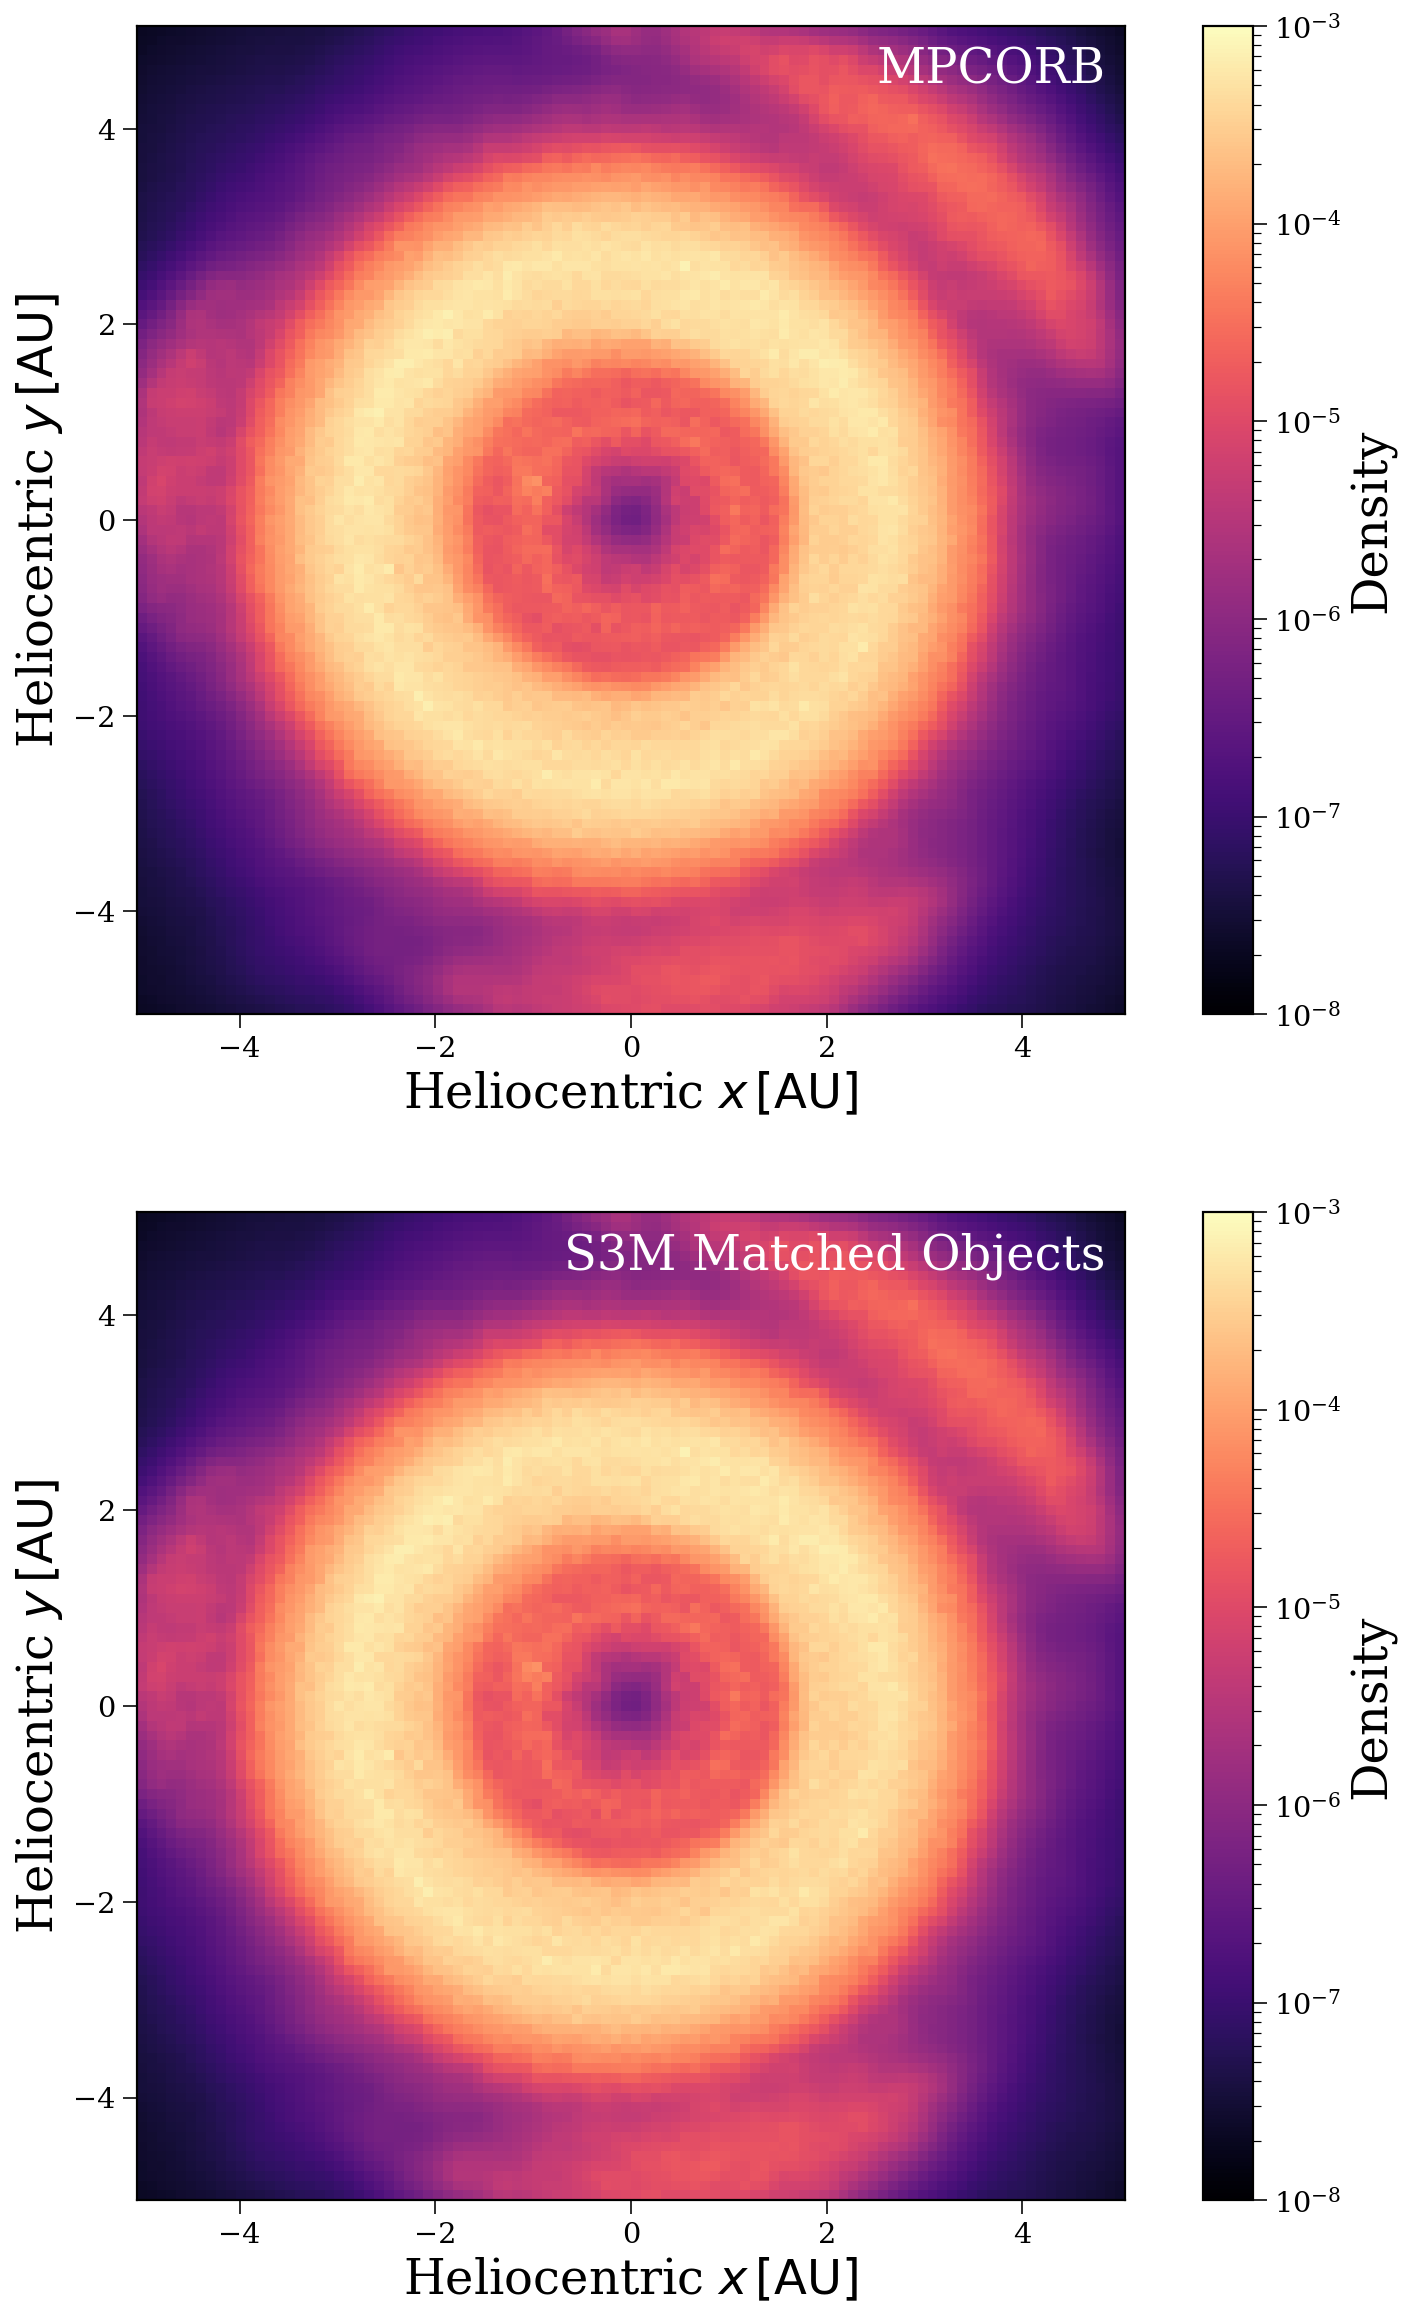
\includegraphics[width=\columnwidth]{density_comparisons.png}
    \caption{A comparison of the density of \mpco{} objects with those objects that were matched in \sss{} by our hybrid catalogue pipeline.}
\end{figure}